
\section{A tutorial walkthrough}
\label{sec:tutorial}

Welcome to the Utool tutorial! In this tutorial, we will walk you
through some of the basic operations that Utool supports.

\subsection{Installation}

Utool is distributed as a Java package with the filename
\verb?Utool-<version>.jar?. After downloading it from the website, you
can simply run it as follows:\footnote{We write ``\texttt{\$ command}''
for commands that you type on a shell; everything else is the output
of the system.}


\begin{verbatim}
$ java -jar Utool-3.0.jar
Usage: java -jar Utool.jar <subcommand> [options] [args]
Type `utool help <subcommand>' for help on a specific subcommand.
Type `utool --help-options' for a list of global options.
Type `utool --display-codecs' for a list of supported codecs.

Available subcommands:
    solve        Solve an underspecified description.
    solvable     Check solvability without enumerating solutions.
    convert      Convert underspecified description from one format to another.
    classify     Check whether a description belongs to special classes.
    display      Start the Underspecification Workbench GUI.
    server       Start Utool in server mode.
    help         Display help on a command.

Utool is the Swiss Army Knife of Underspecification (Java version).
For more information, see www.coli.uni-sb.de/projects/chorus/utool/
\end{verbatim}
%$

This assumes that you have installed Java 5.0 or higher and it is in
your path. You can move the Jar to any directory you like and then
pass the pathname of the file to Java. You could also define an shell
alias for calling Utool more conveniently if you like, e.g. as
follows (on a bash shell):

\begin{verbatim}
$ alias utool='java -jar /usr/local/Utool-3.0.jar'
$ utool
Usage: java -jar Utool.jar <subcommand> [options] [args]
Type `utool help <subcommand>' for help on a specific subcommand.
Type `utool --help-options' for a list of global options.
Type `utool --display-codecs' for a list of supported codecs.
...
\end{verbatim}

For the rest of this tutorial, we will only write \verb?utool? for
the call to the Utool main program, for easier readability. You can
either define the alias, or expand \verb?utool? to the appropriate
\verb?java -jar Utool-3.0.jar? call yourself.

Next to the compiled Java classes, the Jar contains a collection of
example files that we will use in this tutorial. You don't usually
need to unpack the Jar to use it, but for the purposes of this
tutorial, start by running the following command:

\begin{verbatim}
$ jar xf Utool-3.0.jar
\end{verbatim}
%$

This will unpack the contents of the Jar file into the current
directory. Most importantly, it will create the directory
\verb?examples?, which contains the example files we will use below.




\subsection{Checking whether an USR is solvable}

First of all, let's use Utool to determine whether a given dominance
graph is solvable. ``Solvable'' means that it is possible to configure
the fragments of the graph (i.e.\ those subgraphs which are connected
by solid ``tree'' edges) into a forest while realising the (dotted)
dominance edges as reachability in the tree. Such a forest-shaped
arrangement of a dominance graph is called a \emph{solved form} (see
Fig.~\ref{fig:chain3}). Many solvable graphs also have
\emph{configurations}, i.e.\ trees that consist only of the labelled
nodes in the dominance graph, connected by tree edges. All this is
defined in detail e.g.\ in \cite{Koller04}.

\begin{figure}
%HEVEA \begin{latexonly}
\centering
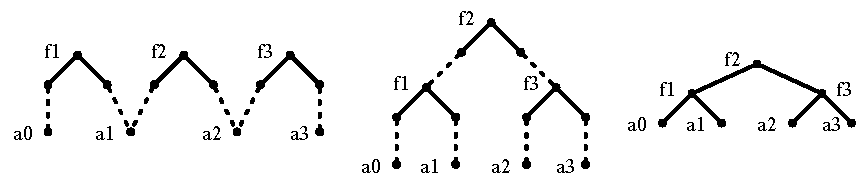
\includegraphics{chain.pdf}
%HEVEA \end{latexonly}
%HEVEA \imgsrc{chain.png}
\caption{The chain of length 3 (left), along with one of its five
solved forms (middle) and one of its configurations (right).
\label{fig:chain3}}
\end{figure}

We will do this for the graph specified in the file
\url{examples/chain-3.clls} (shown in Fig.~\ref{fig:chain3}). This
graph is in fact solvable, and has five solved forms.

The Utool command for checking solvability is called
\verb?solvable?. Thus you can check the example graph for solvability
as follows:

\begin{verbatim}
$ utool solvable -s examples/chain-3.clls
The input graph is normal.
The input graph is compact.

Solving graph ... it is solvable.
Splits in chart: 10
Time to build chart: 60 ms
Number of solved forms: 5
\end{verbatim}
%$

The output states that the graph is solvable and has five solved
forms. It also contains some information about the input graph (it is
normal and compact), the chart data structure computed by the solver
(it contains ten splits), and the time it took to compute the
chart. In addition, the program terminated with an exit code of 1 to
signal that the graph was indeed solvable. If you ran Utool from a
bash shell, you can display this exit code with the command
``\verb!echo $?!''. %$

As you can see, the Utool command line consists of four parts:
\begin{itemize}
\item \verb?utool? (or \verb?java -jar Utool-3.0.jar?): This instructs
Java to load the Jar file and run its main class. You can pass further
arguments to the Java VM by putting them before the \verb?-jar?
option.
\item \verb?solvable?: Most of the time, a call to Utool will contain
exactly one \emph{command}. There are seven commands --
\verb?solvable?, \verb?solve?, \verb?convert?, \verb?classify?,
\verb?display?, \verb?server?, and \verb?help? -- which perform
different tasks. We will walk you through all seven commands here, and
then describe them in more detail in Section~\ref{sec:operations}.
\item \verb?-s?: After the command, you can specify \emph{options}. In
this case, we selected one option (\verb?-s? or
\verb?--display-statistics?), which was responsible for printing all
the output from the example run above. We could have left the option
away; then the Utool run would have done exactly the same, and
returned the same exit code, but it wouldn't have printed these
informational messages.
\item \verb?examples/chain-3.clls?: This is the name
of the file from which the dominance graph should be read. The file
can contain a direct specification of a dominance graph (as in this
case), or it can contain an USR of some other underspecification
formalism which is then translated to a dominance graph
automatically.
\end{itemize}



\subsection{Enumerating solutions}

Now that we know that the dominance graph is solvable, let's have
Utool show us the five solved forms that it claimed exist. We do this
using the \verb?solve?  command, like so:

\begin{verbatim}
$ utool solve -O term-prolog examples/chain3.clls
f1(a0,f2(a1,f3(a2,a3)))
f1(a0,f3(f2(a1,a2),a3))
f2(f1(a0,a1),f3(a2,a3))
f3(f2(f1(a0,a1),a2),a3)
f3(f1(a0,f2(a1,a2)),a3)
\end{verbatim}
%$

The five solved forms of the graph are displayed as terms in Prolog
syntax: Utool transforms each solved form into a \emph{configuration}
by identifying roots and holes as shown in Fig.~\ref{fig:chain3}, and
then prints the resulting trees as ground terms. You may want to
convince yourself at this point that the graph indeed has exactly five
solved forms, and that the five terms shown above are such term
representations of the configurations.

We had to use a new command-line option in the \verb?solve? command:
\verb?-O term-prolog? (which is shorthand for
\verb?--output-codec term-prolog?). Once Utool has computed a solved
form, it needs to know how it should translate this solved form into a
string representation. This translation is handled by an \emph{output
codec}. A number of output codecs are distributed with Utool; you can
also implement your own output codec if you like. In the example, we
used the \verb?term-prolog? output codec, which maps solved forms into
configurations and these configurations into Prolog terms as explained
above.

Speaking of codecs: There are also \emph{input codecs}, which map from
a string representation of an USR into a dominance graph. In the
example, Utool read the string representation from the file with the
specified name (\url{chain3.clls}) and passed it to an input codec to
obtain a dominance graph from it. In this case, we didn't have to
specify the input codec explicity, because Utool knows that the
filename extension \verb?.clls? is associated with the
\verb?domcon-oz? input codec, and used this codec automatically. We
could also have specified the input codec explicitly using the
\verb?-I domcon-oz? or \verb?--input-codec domcon-oz? option. Codecs
can be much more powerful than the ones mentioned here, and are
described in depth in Section~\ref{sec:codecs}.

 
\subsection{Converting and classifying USRs}

Utool works with labelled dominance graphs internally; input codecs
are used to translate from other formalisms into labelled dominance
graphs, and output codecs are used to translate from labelled
dominance graphs into other formalisms. These translations can be
non-trivial, and we have defined and proven them correct in several
research papers \cite{KolNieTha03,mrs-dom}.

A special case is if you make Utool read a USR in some formalism,
which it translates into a labelled dominance graph, and then output
this same labelled dominance graph using a different output
codec. What this does is essentially to convert a USR into an
equivalent USR in some other formalism. This allows you to use our
theoretical groundwork on formal translations between
underspecification formalisms in a convenient way, and can be useful
in certain situations.

Let's look at an example again. The file
\url{examples/rondane-1.mrs.pl} is an USR in the
Minimal Recursion Semantics formalism \cite{CopFliSag97}. This MRS is
computed by the English Resource Grammar
\cite{Copestake&Flickinger:LKB} for the first sentence in the Rondane
Treebank, which is distributed with the ERG. Its filename extension is
\verb?.mrs.pl?, which is associated with the \verb?mrs-prolog? input
codec. Now let's convert this MRS into a labelled dominance graph in
Oz syntax (output codec \verb?domcon-oz?).

\begin{verbatim}
$ utool convert examples/rondane-1.mrs.pl -O domcon-oz
%% autogenerated by Utool 3.0 (see www.coli.uni-sb.de/projects/chorus/utool for details)
[label(h54 named) label(h51 proper_q(h52 h53)) label(h45 '_of_p&_part_n&_and_c'(
h43 h47)) label(h47 '_western_a') label(h43 '_eastern_a') label(h40 '_the_q'(h42
 h41)) label(h36 '_between_p&_route_n&_main_a') label(h33 '_the_q'(h35 h34)) lab
el(h25 '_of_p_sel&card&part_of') label(h27 def_explicit_q(h28 h29)) label(h23 '_
once_a'(h24)) label(h21 '_be_v_id') label(h10 '_valley_n&compound&_and_c'(h8 h12
)) label(h19 named) label(h16 proper_q(h17 h18)) label(h12 '_historic_a') label(
h8 '_well+known_a') label(h4 '_the_q'(h7 h5)) label(h1 prpstn_m(h3)) dom(h52 h54
) dom(h42 h45) dom(h35 h36) dom(h28 h25) dom(h24 h21) dom(h17 h19) dom(h7 h10) d
om(h3 h23) dom(h3 h33) dom(h3 h16) dom(h3 h27) dom(h3 h40) dom(h3 h51) dom(h3 h4
) dom(h34 h25) dom(h18 h10) dom(h29 h21) dom(h41 h36) dom(h53 h45) dom(h5 h21)]
\end{verbatim}
%$


In addition, Utool can check for you whether the labelled dominance
graph it works with belongs to one of a number of important classes
using the \verb?classify? command, like so:

\begin{verbatim}
$ utool classify -s examples/rondane-1.mrs.pl
The input graph is normal.
The input graph is not compact, but I will compactify it for you.
The graph is hypernormally connected.
The graph is leaf-labelled.
\end{verbatim}
%$

Among other things, Utool just told us that the graph is
\emph{hypernormally connected} and \emph{leaf-labelled}
\cite{KolNieTha03}. This is very important because USRs written in MRS
or Hole Semantics can only be correctly encoded into a labelled
dominance graph if the resulting graph has these two properties; the
technical reason for this is that we can guarantee that every solved
form has a configuration only for such graphs. We hypothesise that all
correct USRs that are currently produced by large-scale grammars are
indeed hypernormally connected and leaf-labelled; using the
\verb?classify? command, we can quickly go through a large number of
USRs from a corpus and test this hypothesis \cite{FliKolTha05}.

One final note is that if you call Utool from a script that does such
batch processing, you can conveniently retrieve the classification by
looking at the exit code of the Utool process. For instance, a bash
shell makes the exit code of the previous process accessible to you in
the \verb!$?! shell variable, so you get the following result:

\begin{verbatim}
$ echo $?
59
\end{verbatim}
%$

The exit code $59 = 32 + 16 + 8 + 2 + 1$ indicates that the graph is
leaf-labelled, hypernormally connected, compactifiable, normal, and
weakly normal, but not compact. These exit codes are documented in
Section~\ref{sec:op-classify} below. 



\subsection{The Underspecification Workbench} 

Utool comes with a graphical user interface (Ubench, the
Underspecification Workbench) which will display labelled dominance
graphs and their solved forms and give you access to all the
functionality that is also available from the command-line tool.

You can start Ubench as follows:
\begin{verbatim}
$ utool display
\end{verbatim}
%$

\begin{figure}
\begin{center}
%HEVEA \imgsrc{ubench.png}
%HEVEA \begin{latexonly}
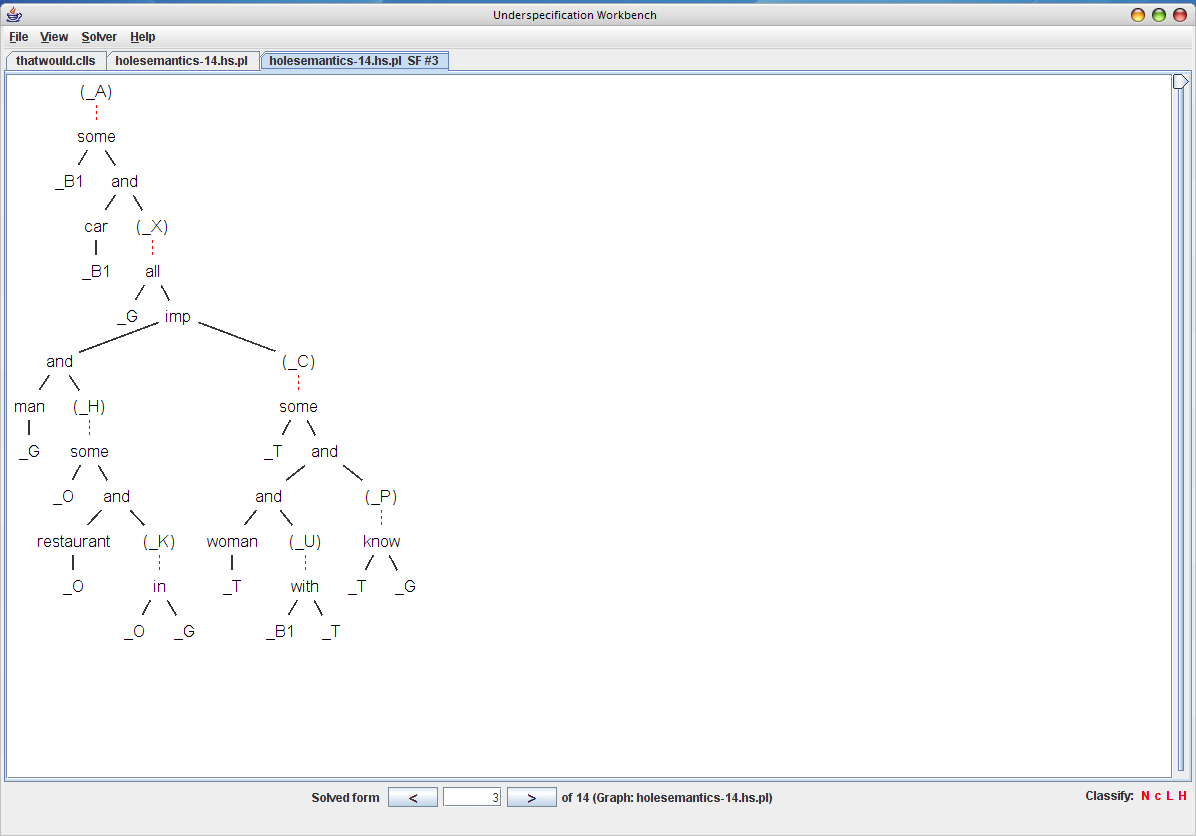
\includegraphics[width=0.8\textwidth]{ubench.png}
%HEVEA \end{latexonly}
\end{center}
\caption{The Underspecification Workbench. \label{fig:ubench}}
\end{figure}


This will bring up the main Ubench window (see
Fig.~\ref{fig:ubench}). At this point, it displays just a menu and an
empty content pane, but you can use the File/Open menu to load
USRs. Alternatively, you can pass the name of an USR file to Ubench
directly as follows:

\begin{verbatim}
$ utool display examples/rondane-1.mrs.pl
\end{verbatim}
%$

This will load the given USR and display it immediately. Notice that
Ubench automatically classifies new USRs it loads, and displays the
results in the lower right corner of the window. It also solves the
USR and displays the number of solved forms. You can then click on the
``Solve'' button to display the first solved form, and then cycle
through the other solved forms from there. In addition, Ubench is able
to export an USR using another output codec (through the File/Export
menu), or export the graph as it is currently drawn as a PDF file
(through the File/Export as PDF menu).



\subsection{The Utool Server} 

The final command we discuss in this tutorial is the \verb?server?
command, which starts Utool in server mode. In server mode, Utool
keeps running indefinitely; it accepts commands via a socket, executes
these commands, and sends the results back through the socket. You can
start Utool in server mode as follows:

\begin{verbatim}
$ utool server
\end{verbatim}
%$

This will open a socket on port 2802 of your machine and listen to
commands sent from this port. If you have Perl installed on your
system, you can test the Utool Server using the demo client we have
included in the distribution. Keep the \verb?utool server? process
running, and execute the following command:

\begin{verbatim}
$ perl tools/client/utool-client.pl solve -I domcon-oz -O term-prolog \
         examples/chain3.clls
f1(a0,f2(a1,f3(a2,a3)))
f1(a0,f3(f2(a1,a2),a3))
f2(f1(a0,a1),f3(a2,a3))
f3(f2(f1(a0,a1),a2),a3)
f3(f1(a0,f2(a1,a2)),a3)
\end{verbatim}

The server supports exactly the same commands as the command-line
version (except that you can't use it to start another
server). However, it has the advantage that you need to run only a
single process to execute any number of commands, whereas you must
start a new Java process for each new command when you use the
command-line tool. This saves runtime if you need to run a large
number of successive commands, such as when classifying all USRs in a
corpus: You don't have the overhead for starting Java, and the
programme will also become faster over time because the Java system
has the opportunity to just-in-time compile the Java bytecode.

The exact operation of the Utool Server is described in
Section~\ref{sec:operations}.







%%% Local Variables: 
%%% mode: latex
%%% TeX-master: "0"
%%% TeX-command-default: "LaTeX"
%%% End: 
